\chapter{Outsider Anonymous Identity-Based Broadcast Encryption}
\label{cha:n}

\section{Online Social Network}
OSNs are getting more and more aware of the rising privacy concerns among their users. Therefore, most OSN services like Google+ and Facebook try to offer preferences that allow the user to determine their privacy up to a certain extent. In practice, most OSNs realise this by offering user specified groups of friends that can be selected when broadcasting a message over the OSNs' network. The OSN provider then ensures that the broadcasted message is only shown to members inside the user specified group. However, these methods are insufficient for most privacy aware users.

\subsection{Definition}
It might be useful to take one step back and define what an online social network actually is. Different definitions have found their way in literature but the most commonly accepted is the definition of a \textit{Social Networking Service} (SNS) from Boyd et al.~\cite{art:BoydE08}

\begin{defn}[Definition of a SNS by Boyd et al~\cite{art:BoydE08}]
\label{def:osn_boyd}
 A \textit{social networking service} (SNS) is a web-based service that allows individuals to:
 \begin{enumerate}
  \item Construct a public or semi-public profile within a bounded system
  \item Articulate a list of other users with whom they share a connection.
  \item View and traverse their list of connections and those made by others within the system
  \setcounter{enumTemp}{\theenumi}
 \end{enumerate}
\end{defn}

Definition~\ref{def:osn_boyd} is at the same time generic enough to cover all kinds of social networking services, as well as specific enough to distinguish SNSs from other web-based applications. However, Definition~\ref{def:osn_boyd} is still too generic for our purposes as we only consider one specific type of SNS, namely the SNSs from Definition~\ref{def:osn_boyd} that offer the ability to broadcast messages. Therefore, an \textit{Online Social Network} (OSN) is redefined in Definition~\ref{def:osn}. For the sake of clarity, from this moment onwards SNS will refer to a Social Networking Service as in Definition~\ref{def:osn_boyd} while OSN will denote an Online Social Network as in Definition~\ref{def:osn}.

\begin{defn}[OSN]
\label{def:osn}
 An \textit{Online Social Network} (OSN) is a social networking service (SNS), that in addition to the possibilities from Definition~\ref{def:osn_boyd} also allows its users to
 \begin{enumerate}
  \setcounter{enumi}{\theenumTemp}
  \item Distribute messages to anyone visiting the system, any user of the system or subsets thereof.
 \end{enumerate}
\end{defn}


\subsection{Model}
\label{sec:model}
\begin{defn}[OSN user]
\label{def:user}
 An \textit{OSN user} $U$ is any entity that has a profile on the OSN and thus identifiable by a unique identifier \id{U}. The set containing all users of an OSN is denoted $\mathcal{U}$.
\end{defn}

An OSN user can perform different activities within the infrastructure of the OSN. Depending on the performed activity, the user is labeled as one of three different roles: a sender, a friend or a recipient.

\begin{defn}[Sender]
\label{def:sender}
 A \textit{sender} $B$ is an OSN user who broadcasts a message $m$ over the OSN infrastructure to varying subsets of OSN users, called the \textit{intended recipient set} $\mathcal{S}$ such that $\mathcal{S} \subseteq \mathcal{U}$.
\end{defn}

\begin{defn}[Intended recipient]
\label{def:recipient}
 An \textit{intended recipient} $R$ of a message $m$ is an OSN user who is explicitly designated by a sender $B$ to be part of the intended recipient set $\mathcal{S}$ of that message $m$. The intended recipient set $\mathcal{S}$ takes the form of a list of \id{}'s uniquely identifying other users' profiles in the OSN infrastructure.
\end{defn}

\begin{defn}[Friend]
\label{def:friend}
 An OSN user who shares a connection with another OSN user $U$ in the OSN infrastructure, is called a \textit{friend of the user $U$}. The set of all friends associated to a user $U$ is denoted $\mathcal{F}_U$ such that $\mathcal{F}_U \subseteq \mathcal{U}$.
\end{defn}

Currently, other entities than OSN users $U \in \mathcal{U}$ associated with a profile $\id{U}$, can access the OSN services as well. Therefore, it is required to define another group of entities called \textit{the viewers}.

\begin{defn}[Viewer]
\label{def:viewer}
 Any virtual or real world entity that is given access to the OSN belongs to the set of viewers $\mathcal{V}$. All viewers with access to the profile $\id{U}$ of a user $U$ are in the set $\mathcal{V}_U \subseteq \mathcal{V}$.
\end{defn}

In modern day OSN infrastructures, many different entities are part of the set of viewers $\mathcal{V}$, i.e. OSN users, advertising companies, system administrators of the OSN, software applications specifically developed for the OSN, etc. Note that these entities do not have to be users neither real life persons. Companies or software code can be part of the set of viewers $\mathcal{V}$ as well. Usually, the OSN determines which entities are member of the set of viewers $\mathcal{V}$. Therefore, the user often has no control in who is a member of $\mathcal{V}_U$. That is, the user $U$ can not determine which entities have access to his profile $\id{U}$.

Figure~\ref{fig:current_model} illustrates previous definitions applied to an OSN as it is often encountered on the internet. The different sets in Figure~\ref{fig:current_model} are defined as follows:
\begin{itemize}
 \item The intended recipient set,
 \begin{equation*}
  \mathcal{S} = \{ \textrm{Recipient 1}, \textrm{Recipient 2} \}
 \end{equation*}
 \item The set of friends of user $B$,
 \begin{equation*}
  \mathcal{F}_B = \{ \textrm{Recipient 1}, \textrm{Recipient 2}, \textrm{Friend 1}, \textrm{Friend 2} \}
 \end{equation*}
 \item The set of viewers who have access to the profile of user $B$,
 \begin{equation*}
  \begin{split}
   \mathcal{V}_B = \{ \textrm{Recipient 1}, \textrm{Recipient 2}, \textrm{Friend 1}, \textrm{Friend 2}, \textrm{Sender } B, \textrm{Advertiser 1}, \\
   \textrm{Application 1} \}
  \end{split}
 \end{equation*}
 \item The set of entities with access to the OSN,
\begin{equation*}
\begin{split}
 \mathcal{V} = \{ \textrm{Recipient 1}, \textrm{Recipient 2}, \textrm{Friend 1}, \textrm{Friend 2}, \textrm{Sender } B, \textrm{Advertiser 1},\\
  \textrm{Application 1}, \textrm{User 1}, \textrm{User 2}, \textrm{Advertiser 2}, \textrm{Application 2} \}
\end{split}
\end{equation*}
\item The set of all users in the OSN,
\begin{equation*}
 \mathcal{U} = \{ \textrm{Recipient 1}, \textrm{Recipient 2}, \textrm{Friend 1}, \textrm{Friend 2}, \textrm{Sender } B, \textrm{User 1}, \textrm{User 2}\}
\end{equation*}
\end{itemize}


\begin{figure}[ht]
    \begin{center}
    \scalebox{0.78}{
        \begin{tikzpicture}[auto, node distance=-2mm, align=center,
            block/.style={rectangle,text width=6em,text centered,minimum height=9mm},
            line/.style={draw,very thick, ->},
            line2/.style={draw,very thick, <->},
            leg/.style={text centered},
            ]
            % Recipient set polygon
            \draw[dashed,color=cyan] (3.5,4) -- (8.5,4) -- (8.5,1.75) -- (3.5,1.75) -- (3.5,4);
            % Friends polygon
            \draw[dashed] (3,4.5) -- (9,4.5) -- (9,-0.25) -- (3,-0.25) -- (3,4.5);
            % Viewers Polygon
            \draw[dashed] (-5,5) -- (9.5,5) -- (9.5,-0.75) -- (-5,-0.75) -- (-5,5);
            % OSN Polygon
            \draw[dashed] (-5.5,5.5) -- (10,5.5) -- (10,-2.75) -- (-5.5,-2.75) -- (-5.5,5.5);
            %\draw[help lines] (-6,-5) grid (8,6);
            \path
                % Images
                (0,3) node [block] (pkg) {
\includegraphics[scale=0.15]{img/bluepkg.png}}
                (-4,3) node [block] (alice) {
\includegraphics[scale=0.15]{img/bluealice.png}}
                (5,3) node [block] (bob) {
\includegraphics[scale=0.15]{img/bluebob.png}}
                (7,3) node [block] (bob1) {
\includegraphics[scale=0.15]{img/bluebob.png}}
                (5,1) node [block] (bob2) {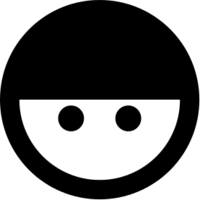
\includegraphics[scale=0.15]{img/bob.png}}
                (7,1) node [block] (alice1) {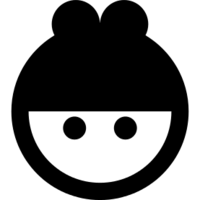
\includegraphics[scale=0.15]{img/alice.png}}
                (-1.5,1) node [block] (adv) {
\includegraphics[scale=0.15]{img/bluemoneyman.png}}
                (1.5,1) node [block] (app) {
\includegraphics[scale=0.15]{img/blueapp.png}}
                
                (1.5,-1.5) node [block] (app2) {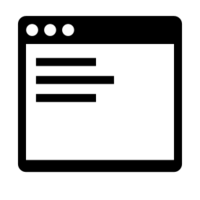
\includegraphics[scale=0.15]{img/app.png}}
                (-1.5,-1.5) node [block] (adv2) {
\includegraphics[scale=0.15]{img/moneyman.png}}
                
                
                (5,-1.5) node [block] (alice2) {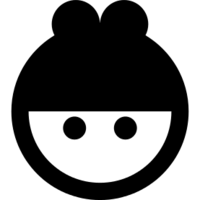
\includegraphics[scale=0.15]{img/alice.png}}
                (7,-1.5) node [block] (bob3) {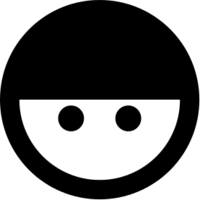
\includegraphics[scale=0.15]{img/bob.png}}
                
                (-1.5,-4) node [block] (spy1) {
\includegraphics[scale=0.15]{img/spy.png}}
                (1.5,-4) node [block] (spy2) {
\includegraphics[scale=0.15]{img/spy.png}}
                % Text
                (0,5.5) node [leg,fill=white] (white_block) {Entities with access to the OSN $\mathcal{V}$}
                (0,5) node [leg,fill=white] (white_block) {Entities with access to $B$'s Profile $\mathcal{V}_B$}
                (6,4) node [color=cyan,leg,fill=white] (white_block) {Intended Recipient Set $\mathcal{S}$}
                (6,4.5) node [leg,fill=white] (white_block) {Friends Set $\mathcal{F}_B$}
                (-2,3.25) node [leg,color=cyan] (white_block) {$m, \mathcal{S}$}
                ;
                
       \node[node distance=2mm, above=of pkg,color=cyan] {\textbf{OSN Broadcast Server}};
       \node[below=of adv,color=cyan] {Advertiser 1};
       \node[below=of adv2] {Advertiser 2};
       \node[below=of app2] {Application 2};
       \node[below=of alice2] {User 1};
       \node[below=of bob3] {User 2};
       \node[below=of bob,color=cyan] {Recipient 1};
       \node[below=of bob1,color=cyan] {Recipient 2};
       \node[below=of bob2] {Friend 1};
       \node[below=of alice1] {Friend 2};
       \node[below=of app2] {Application 2};
       \node[below=of alice,color=cyan] {Sender $B$};
       \node[below=of app,color=cyan] {Application 1};
       \node[node distance=-6mm,below=of spy1] {Outsider 1};
       \node[node distance=-6mm,below=of spy2] {Outsider 2};
       \begin{scope}[every path/.style=line,color=cyan]
        \path (alice.east) -- (pkg.west);
        %\path (pkg.south west) -- (adv.north);
        \path (-0.7, 2.3) -- (adv.north);
        \path (0.7,2.3) -- (app.north);
        \path (pkg.east) -- (3.5,3);
       \end{scope}


        \end{tikzpicture}
    }
    \end{center}
    \caption{Model of the current OSN situation}
    \label{fig:current_model}
\end{figure}

Figure~\ref{fig:current_model} illustrates the situation in which Sender $B$ wants to broadcast a message over the OSN infrastructure to the intended recipient set $\mathcal{S}$. As Sender $B$ only wants to share her message with a specific group of friends, she defines the intended recipient set such that $\mathcal{S} \subset \mathcal{F}_B$. Next, she sends the message $m$ to the OSN's distribution server along with the intended recipient set $\mathcal{S}$. The OSN Server further distributes the message to all users in the recipient set $\mathcal{S}$. Also a subset of third party applications and advertisers get access to the distributed message if they are inside the viewers group $\mathcal{V}_B$. Every entity who has access to the message is coloured blue in Figure~\ref{fig:current_model}.

The infrastructure of the OSN stores almost everything within the viewer set $\mathcal{V}$. The profiles of all users within the friends set $\mathcal{F}_B$, the list of \id{}'s within the intended recipient set $\mathcal{S}$, access rights of applications and advertisers that are part of $\mathcal{V}_B$ and access rights of entities within the set $\mathcal{V}$ are all explicitly stored somewhere on the servers of the OSN. The OSN broadcast server in Figure~\ref{fig:current_model} only models one specific task of the OSN, i.e. broadcasting messages $m$ to every entity who should have access to the message $m$.

Note that not all OSNs support the functionality to define intended recipient sets $\mathcal{S}$ on a per message basis. In OSNs like Twitter the standard privacy settings are such that message are always published publicly. Therefore, the model from Figure~\ref{fig:current_model} only holds for a specific subset of OSNs like Facebook or Google+. More public OSNs like Twitter would require less sets of entities to model their behaviour.

It requires almost no additional effort to transform the model from Figure~\ref{fig:current_model} such that it also takes the sharing of other media than messages into account. The model could then adopted for use on SNSs like Youtube or Instagram as well. However, this falls out of the scope of this thesis.

\subsection{Problem Statement}
\label{sec:problem_statement}
The situation illustrated by Figure~\ref{fig:current_model} might raise the eyebrows of a critical reader since there are several issues with the current OSN situation as modelled in Figure~\ref{fig:current_model}.

First, there is a clear mismatch between the expectations of Sender $B$ and the functionality of the OSN. When a privacy-aware user like sender $B$ takes the effort to define an intended recipient set $\mathcal{S}$, she expects to have full control on who has access to her messages $m$. In reality, sender $B$ only has partial control since the OSN determines all other entities in $\mathcal{V}_B$ that are not part of sender $B$'s friend list $\mathcal{F}_B$. In some OSNs a user first has to give permission to third party applications before access is granted to the user's content. Note that this gives more control to OSN users on determining who is inside the viewers set $\mathcal{V}_B$. Nevertheless, in practice it is still hard to get a concise overview from the OSN on everyone inside $\mathcal{V}_B$.

Second, any user broadcasting messages over the OSN infrastructure has to trust the OSN that it effectively operates as claimed. If the OSN broadcast server in Figure~\ref{fig:current_model} would accidentally broadcast messages publicly despite of the sender's privacy settings, it would be hard for the Sender to find out.

Furthermore, the users of the OSN have to rely on the security of the OSN's infrastructure. If one of the outsiders in Figure~\ref{fig:current_model} would succeed in hacking the OSN's digital infrastructure, he would have immediate access to all sensible information stored on the OSN's servers. Similarly, governments can subpoena the OSN to disclose sensible information on certain users with the argument of national security.

Another significant point is that the OSN fully determines which access policies are supported. As already mentioned in Section~\ref{sec:model}, not all OSNs offer the definition of an intended recipient set on a per message basis. Even OSNs currently supporting this functionality can suddenly stop offering the service. Moreover, nothing prevents OSN providers from changing their privacy policy on a regular basis, thereby complicating users to define the access policy of their choice.

Besides the earlier mentioned issues, the OSN often operates with a corporate mentality. The OSN has no initiative to stop adding advertisers and applications to the set of entities with access to a user's profile $\mathcal{V}_B$. The more information advertising companies receive from the OSN provider, the better they can tailor advertisements to the user. The more third party applications rely on the OSNs infrastructure, the more appealing the OSN business model looks like. Therefore, OSNs have often no initiative to offer stricter access control policies to their users.

\subsection{Existing Solutions}
\label{sec:existing_solutions}
Several existing solutions have been proposed in literature, all trying to solve most of the earlier mentioned issues in OSNs.

\paragraph{flyByNight~\cite{art:LucasB09}} is a Facebook application that protects user data by storing it in encrypted form on Facebook. It relies on Facebook servers for its key management and is therefore not secure against active attacks by Facebook itself.

\paragraph{NOYB (None Of Your Business)~\cite{art:GuhaSTF08}} replaces the details of user $A$ with those of random users $B$ and $C$ thereby making this process only reversible by friends who are allowed to see the profile of user $A$. However this can not be applied to user messages or status updates that are the most frequently used features in the OSNs considered in this thesis.

\paragraph{FaceCloak~\cite{art:LuoXH09}} stores published Facebook data on its servers in encrypted form and replaces the data on Facebook with random text fetched from Wikipedia. This could be a useful mechanism to prevent OSNs from blocking security aware users because they are scared to see their advertising revenues shrink. However, this approach has the disadvantage that other users could take this data to be genuine user content. Furthermore, FaceCloaks architecture leads to an inefficient key distribution system.

\paragraph{Persona~\cite{art:BadenBSBS09}} is a scheme that can be used as a Firefox extension to let users of an OSN determine their own privacy by supporting the ability to encrypt messages to a group of earlier defined friends based on \textit{attribute-based encryption (ABE)}\cite{art:SahaiW04}. The scheme supports lots of useful use cases such as sending messages to all friends that are related to a certain attribute or even encrypting messages to friends of friends. The major drawback of this system however is that every new friend has to exchange a public key before he is able to interact in the privacy preserving architecture consequently requiring an infrastructure for broadcasting and storing public keys. Furthermore, to support the encryption of messages to friends of friends, user defined groups should be made available publicly thereby making the public key distribution system even more complicated. Finally the proposed ABE encryption scheme is 100 to 1000 times slower than a standard RSA operation~\cite{art:BadenBSBS09}.

\paragraph{Scramble~\cite{art:BeatoKW11}} is a Firefox extension that allows defining groups of friends that are given access to certain social network updates. The tool uses public key encryption based on OpenPGP~\cite{rfc4880} to broadcast encrypted messages on almost any platform. Furthermore Scramble provides the implementation of a tiny link server such that OSN policies not allowing to post encrypted data are bypassed. However, as indicated by usability studies~\cite{art:WhittenT99} OpenPGP has a higher usage threshold because an average user does not manage to understand OpenPGP properly. Additionally, Scramble has to rely on the security decisions of the web of thrust. It therefore inherits the unpleasant property of OpenPGP that the user can not be sure that the used PGP key actually belongs to the intended Facebook profile.

The most unattractive property of all the above applications is that they have to rely on a rather complex infrastructure. Persona has to support an extended public key distribution system and Scramble relies on the leap-of-faith OpenPGP web of trust. All proposed solutions require users with no cryptographic background on asymmetric cryptography to make responsible decisions concerning the management of their keys. Furthermore, maintaining such complex key infrastructures gets more and more complex as more users subscribe.

\section{Goals}
The goal of this thesis is to develop an architecture that circumvents the issues discussed in Section~\ref{sec:problem_statement} thereby taking the challenges and pitfalls from earlier solutions in Section~\ref{sec:existing_solutions} into account. Specifically the architecture should have the following properties:
\begin{itemize}
 \item \textbf{User friendly:} An average OSN user should be able to use the resulting architecture, i.e. a user with no knowledge on cryptographic primitives.
 \item \textbf{Applicable:} The original OSN environment should not be altered since some OSN providers are probably not willing to support a more confidential architecture because it could possibly hurt their business model.
 \item \textbf{Ready to use:} No additional registration or subscription to third party key architectures should be required to enable usage of the system. As soon as a user subscribes to the OSN provider he should be able to start receiving confidential messages.
\end{itemize}

The following cryptographic goals should be achieved when publishing a message $m$ to a set of intended recipients $\mathcal{S}$ on the OSN with help of the designed architecture:
\begin{itemize}
 \item \textbf{Confidentiality:} The message is protected from disclosure to unauthorised parties, i.e. all entities that are not explicitly in the recipient set $\mathcal{S}$.
 \item \textbf{Authenticity:} The recipients of the message have reasonable assurances of the message's origin.
 \item \textbf{Integrity:} The recipients are assured the message is distributed in its original form as posted by the sender.
 \item \textbf{No redundancy:} The message should be published only once to reach every recipient in the intended recipient set $\mathcal{S}$.
 \item \textbf{Outsider recipient anonymity:} The intended recipients of a broadcasted message should be anonymous to anyone not included in the intended recipient set $\mathcal{S}$. This implies that also the OSN does not have to know who the recipients are. (See also Definition~\ref{def:outsider_anonymity} about outsider-anonymity).
\end{itemize}




\section{Security Model}

\subsection{Threat Model}

\section{Proposed Scheme}

\subsection{Scheme}

\subsection{Evaluation}

\section{Conclusion}

%%% Local Variables: 
%%% mode: latex
%%% TeX-master: "thesis"
%%% End: 
